\section{Summary of results and price-performance}\label{resultsSummary}

In this section we summarize the results obtained using the different configurations presented previously. We discuss the total execution times and monetary costs. Additionally, we introduce an adapted version of the TPC-DS metric to facilitate performance comparisons, which enables us to derive price-performance criteria. Finally, we estimate the cost effects of opting for spot EC2 instances instead of on-demand instances.

\subsection{Total execution times}\label{resultsSummaryTotalExecutionTimes}

Figure \ref{fig:resultsSummaryTotalTimes} presents the total time required for executing the TPC-DS Benchmark at the 1 TB scale factor for the different configurations that we have covered. The total times are composed from the Data Loading Test, the Power Test, and the Throughput Test times. By far the largest component is the Throughput Test in all cases.

\begin{figure}
   \begin{center}
   \scalebox{0.75}{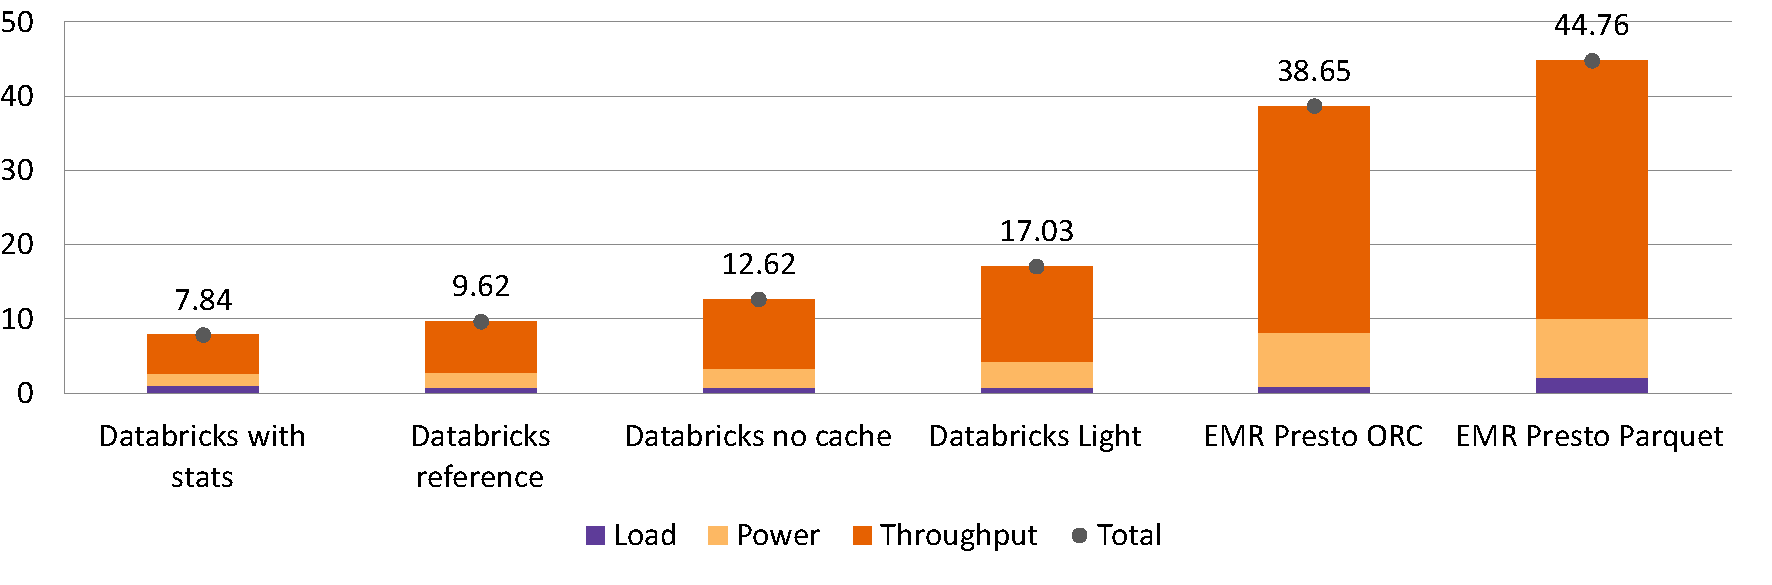
\includegraphics[width=7.0in]{../imgs/resultsSummary/TotalTimes.pdf}}
   \end{center}
   \caption{TPC-DS Benchmark total execution time for various configurations.}
   \label{fig:resultsSummaryTotalTimes}
\end{figure}

The lowest total time is achieved with Databricks using the cost-based optimizer with table and column statistics. It represents an almost 5 times faster alternative than the most efficient configuration for EMR Presto. In the case of Databricks Data Engineering without the cost-based optimizer, our reference configuration, the advantage drops to about 4 times faster, still very significant. Notably, Databricks Light and EMR Presto using the ORC format show very similar performance.

\subsection{Total costs}\label{resultsSummaryTotalCost}

Regarding the monetary costs incurred to obtain the total execution times listed above, we present them in Figure \ref{fig:resultsSummaryTotalCosts}.

\begin{figure}
   \begin{center}
   \scalebox{0.75}{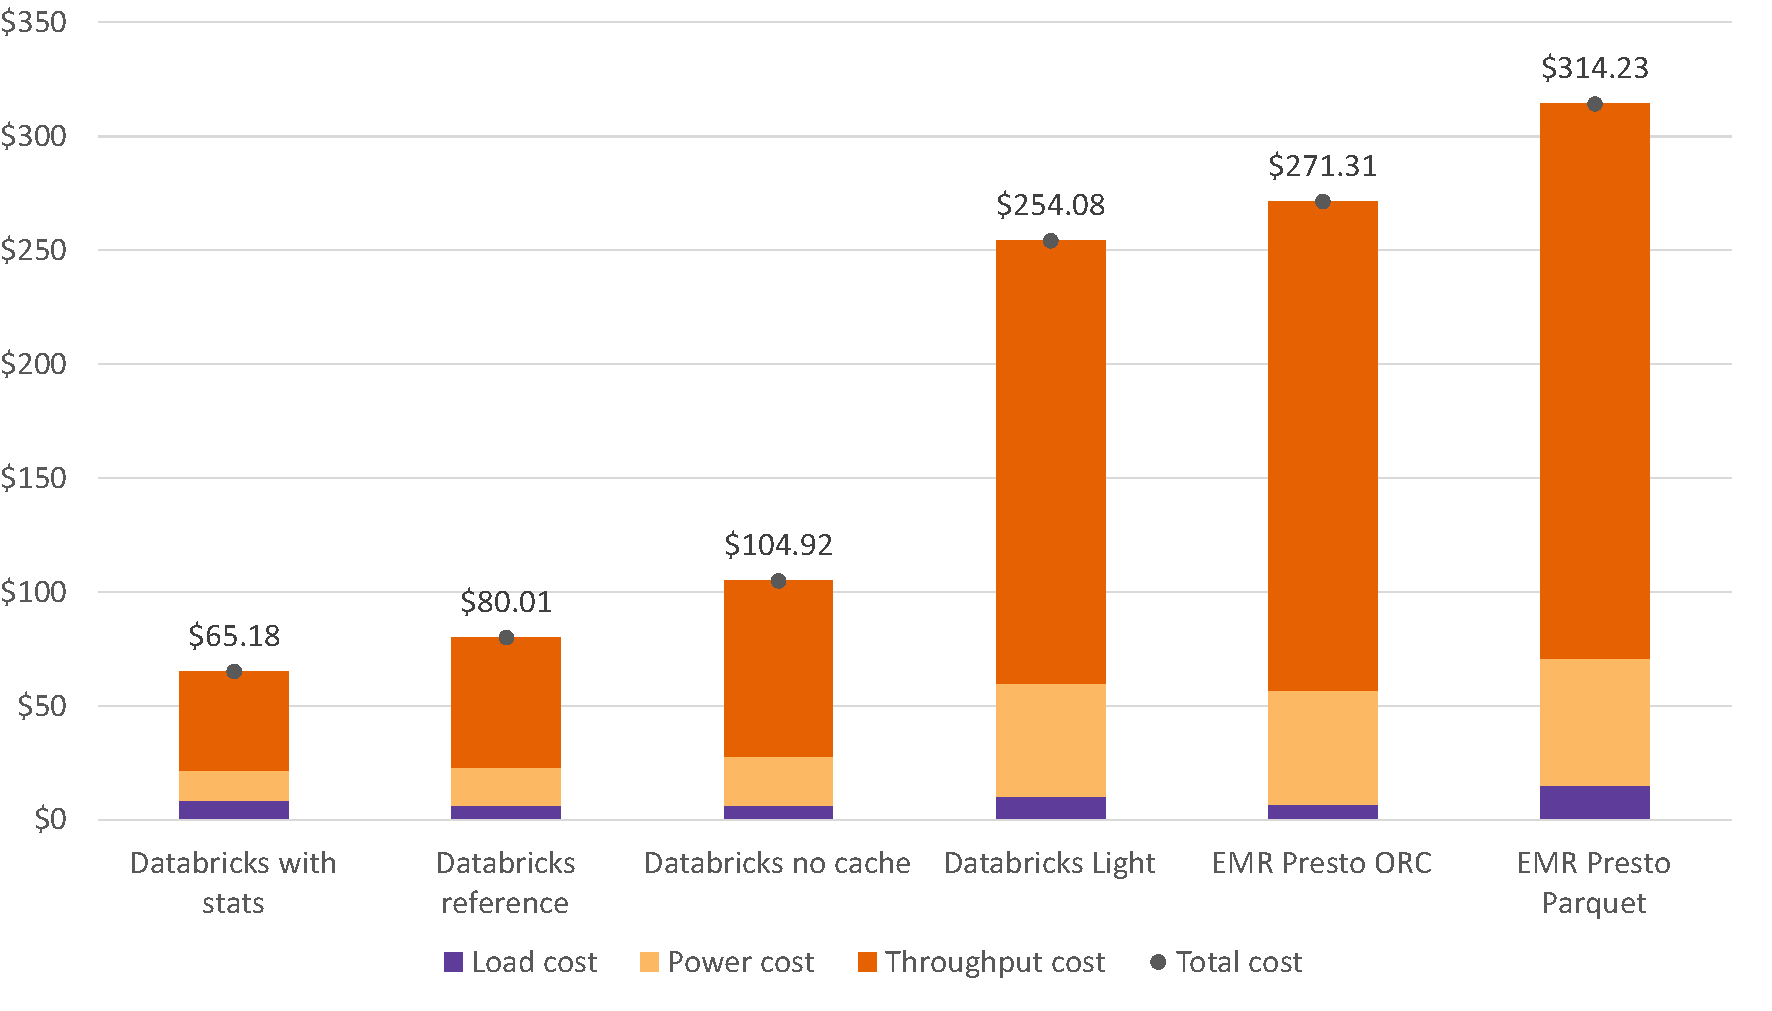
\includegraphics[width=7.0in]{../imgs/resultsSummary/TotalCosts.pdf}}
   \end{center}
   \caption{TPC-DS Benchmark total execution time for various configurations.}
   \label{fig:resultsSummaryTotalCosts}
\end{figure}

Again, we obtain the lowest cost with Databricks with table and column statistics, which is over 4 times cheaper than EMR Presto using ORC. When comparing the reference Databricks configuration with EMR Presto using ORC, it is about 3.4 times cheaper. In turn, Databricks Light is not only slightly faster than EMR Presto ORC, but also cheaper.

Disabling the io cache for Databricks increases the cost significantly, therefore it is a feature that provides real benefits. Nevertheless, additional experiments would be required to determine whether if using lower cost EC2 instances not optimized for io, and potentially inviable for the io cache, could yield a lower cost. For example, the memory optimized r5.2xlarge instances offer the same 8 cores with 3 additional GB of memory, but no NVMe SSD at a cost of \$0.504. Assuming the total time obtained with these instances would be the same as with the cache disabled, the total cost would be \$91.29, still greater than the \$80.01 cost with Databricks Data Engineering with cache enabled, our reference configuration.

The prices shown above employ on-demand EC2 instances. Amazon Web Services offers an alternative pricing model for EC2 instances called spot instances. These represent spare computing capacity that AWS makes available at heavily discounted prices, but whose availability can vary greatly during the year and across the various regions. Furthermore, such changes in availability can trigger spot instance interruptions, which the application should be prepared to handle.

We next estimate the costs of employing spot instances instead of on-demand instances. We base our calculations on the Spot Instance Advisor\footnote{https://aws.amazon.com/ec2/spot/instance-advisor/}, which estimates savings based on data covering the last 30 days. For the i3.2xlarge instances that we use for both our Databricks and EMR Presto deployments, running in the US West (Oregon) region, the savings are reported to be 70\% and the frequency of interruption less than 5\%. This results in the costs we show in Figure \ref{fig:resultsSummaryTotalCostsWithDiscount}.

\begin{figure}
   \begin{center}
   \scalebox{0.75}{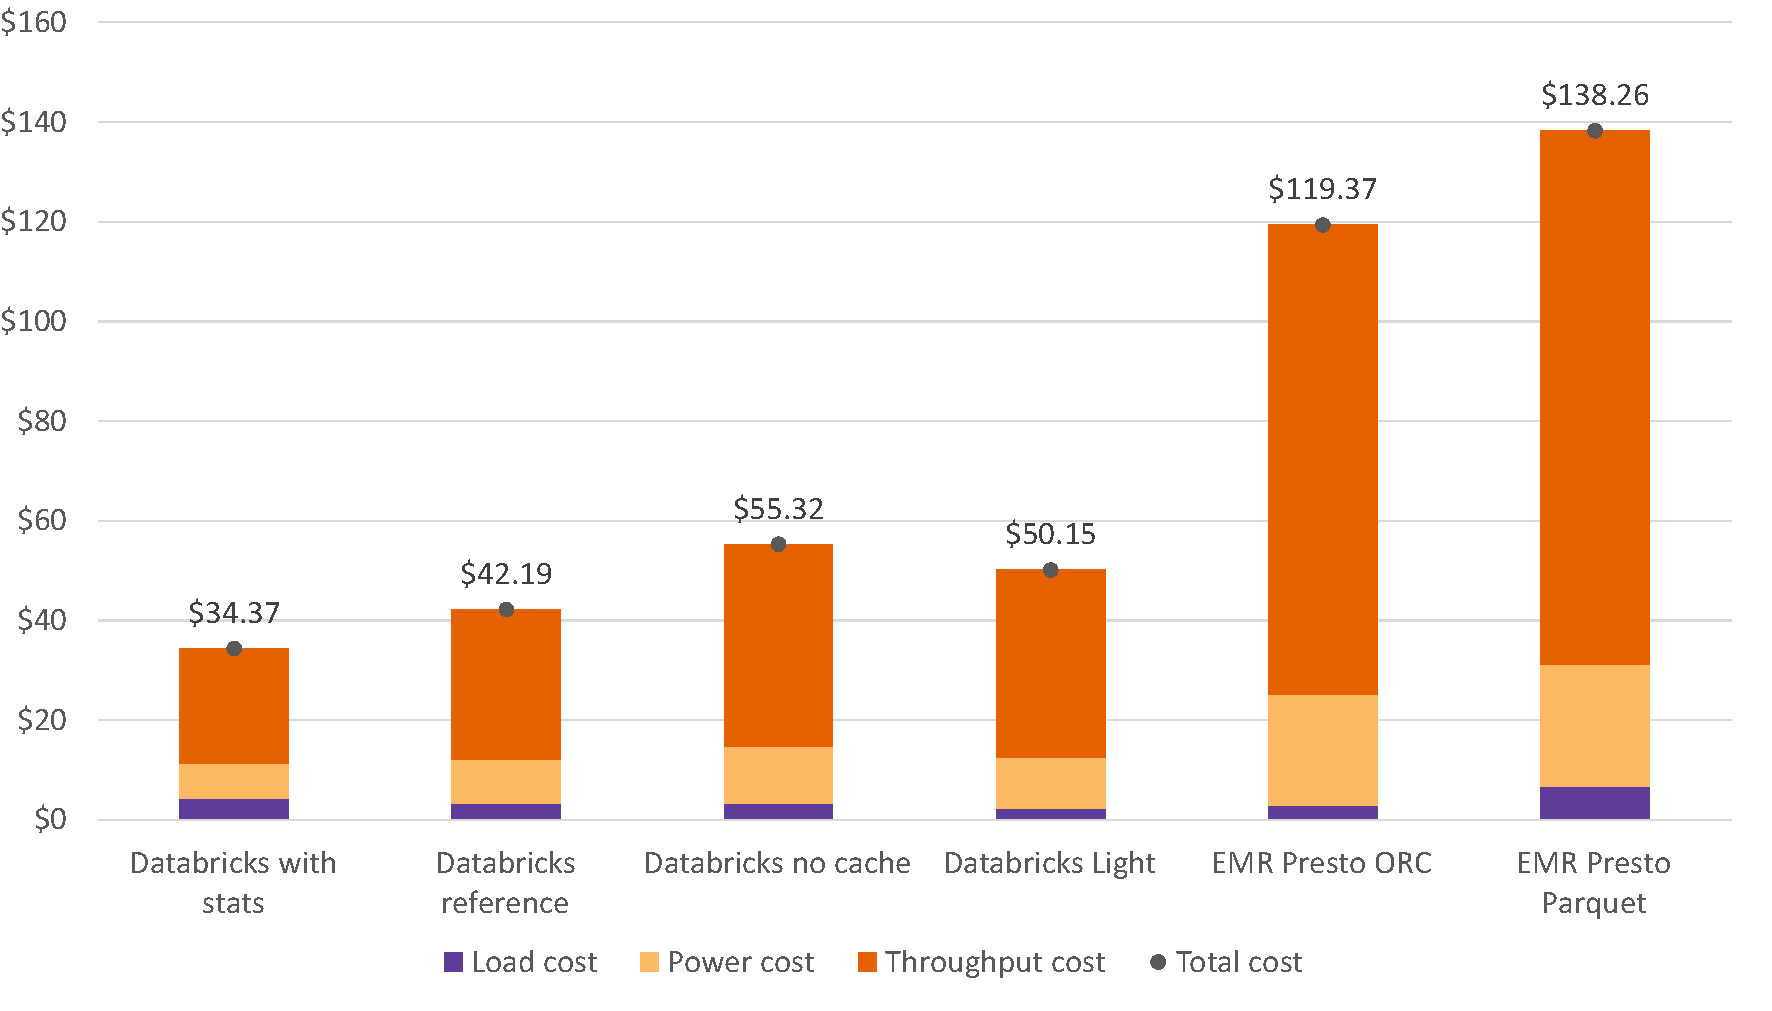
\includegraphics[width=7.0in]{../imgs/resultsSummary/TotalCostsWithDiscount.pdf}}
   \end{center}
   \caption{Estimated TPC-DS Benchmark total cost for various configurations using spot EC2 instances.}
   \label{fig:resultsSummaryTotalCostsWithDiscount}
\end{figure}

The costs are reduced by more or less about half. Since the Databricks Data Engineering software costs now dominate the node cost per hour, the Databricks reference costs compared to the EMR Presto ORC costs now are about 2.8 times cheaper instead of 3.4 times cheaper, still a difference of great magnitude.

\subsection{TPC-DS performance metric}\label{resultsSummaryPerformanceMetric}

The TPC-DS Benchmark defines a performance metric that combines the number of queries and the execution times of the different tests, while also taking the scale factor into consideration. We provide in Equation \ref{eq:TPCDSperfMetric} the formula used to calculate this metric.

\begin{equation}\label{eq:TPCDSperfMetric}
  QphDS@SF = \left\lfloor\frac{SF \cdot Q}{\sqrt[4]{T_{PT} \cdot T_{TT} \cdot T_{DM} \cdot T_{LD}}}\right\rfloor
\end{equation}

Where the components of the QphDS@SF metric are:
\begin{itemize}
\item	$SF$: the scale factor, 1000 for 1 TB in our case.
\item	$Q$: the total number of weighted queries, 99 (number of queries in the benchmark) times the number of streams in the Throughput Test, which is 4 in our experiments.
\item	$T_PT$: the total time to compute the Power Test multiplied by the number of streams.
\item	$T_TT$: total time for the two phases of the Throughput Test, we perform only one phase.
\item	$T_DM$: total time for the two Maintenance Tests, which we do not perform.
\item	$T_LD$: the total time of the Data Loading Test, multiplied by the number of streams and an adjustment factor of 0.01.
\end{itemize}

We do not perform the Data Maintenance Tests and consequently do a single Throughput Test because we address the scenario in which a distributed file system works on an append-only mode. Therefore, we have to adjust the performance metric to the form it takes in Equation \ref{eq:modifiedTPCDSperfMetric}.

\begin{equation}\label{eq:modifiedTPCDSperfMetric}
  QphDS@SF = \left\lfloor\frac{SF \cdot Q}{\sqrt[3]{T_{PT} \cdot T_{TT} \cdot T_{LD}}}\right\rfloor
\end{equation}

Using that equation, we derive the results we present in Figure \ref{fig:performanceMetricResults}.

\begin{figure}
   \begin{center}
   \scalebox{0.75}{\includegraphics[width=7.0in]{../imgs/resultsSummary/performanceMetricResults.pdf}}
   \end{center}
   \caption{TPC-DS Benchmark performance metric for various configurations.}
   \label{fig:performanceMetricResults}
\end{figure}

In this case, a larger number is better, and Databricks with statistics obtains the best score, followed by the reference configuration that does not employ them. Interestingly, Databricks Light obtains a slightly lower score than EMR Presto using ORC, despite having obtained a lower total execution time. This is because EMR Presto using the ORC format was about 50\% more efficient in loading the data. The geometric mean component of the formula makes the corresponding factor more relevant.

From the TPC-DS Benchmark performance metric and the total monetary costs data, we can derive a price-performance metric. In fact, TPC-DS already defines such a metric as simply the price to run the benchmark divided by the score. In our case, we consider the EC2 instances costs and the software costs. The AWS S3 storage costs are not included, but we do not expect them to vary significantly between the two systems. We do not give a monetary cost to the administrative and software development tasks required to create and run the benchmark applications, but we do comment on them in Section \ref{usability}.

In Figure \ref{fig:pricePerformanceResults} we present the price-performance metric for the various system configurations.

\begin{figure}
   \begin{center}
   \scalebox{0.75}{\includegraphics[width=7.0in]{../imgs/resultsSummary/pricePerformanceResults.pdf}}
   \end{center}
   \caption{TPC-DS Benchmark price-performance for various configurations.}
   \label{fig:pricePerformanceResults}
\end{figure}

In this case, a higher value indicates that more money needs to be spent for each benchmark performance unit. Again, Databricks with statistics obtains the best result, closely followed by its alternative configurations. EMR Presto using the ORC format beats Databricks Light, due to the previously discussed higher benchmark score and similar operational costs. The advantages of the ORC format for EMR Presto are also highlighted in comparison to Parquet.




